\chapter{隐私保护k-means聚类方法研究}

\section{引言}
%搬运开题报告
随着现代社会数字化的不断演进,数据使用量呈指数级增加,个人和小型组织越来越难以在内部计算机服务器上维护所有重要信息、运行大型程序和系统。为解决这些问题,云计算应运而生。自云计算在2006年被提出后,它就被认为是能够推动下一代互联网革命的技术,并迅速成为了研究领域的热门话题\cite{sadiku2014cloud}。近年来,随着研究的发展和设备的进步,机器学习从学术研究落地到生活的方方面面,但是大多数机器学习任务对于设备的性能要求较高,需要存储海量的数据才能取得较好的结果。大型公司有能力承担设备费用,利用机器学习的便利开展各种各样的服务,但是资源受限的小公司和个人的需求常常难以被满足。

为解决上述问题,云计算场景下出现了一种新的服务类型-MLaaS,即“机器学习即服务(Machine Learning as a Service)”,它使得技术可以扩展,并且价格合理\cite{ribeiro2015mlaas}。在MLaaS中,海量的数据需要被上传到云计算中心,这一过程也被称之为外包计算。由于用户在数据上传后失去了对数据的完全控制,因此会更加关心隐私安全问题。同时云计算服务模型的复杂性、实时性,数据的多元异构特点以及终端资源有限,传统的数据安全隐私和隐私保护方法无法直接用来保护云计算中的大量数据\cite{hunt2018chiron}。

聚类(Clustering)是一种非常流行的无监督机器学习技术,它了能够将相似的输入元素划分到同一个簇(cluster)中。聚类的应用领域非常广泛,从业务分析到医疗保健等诸多领域。在许多这些应用场景中,敏感信息在被正确聚类的同时,也不应该被泄漏。此外,现在经常需要将不同来源的数据组合起来进行训练以提升分析质量,庞大的数据量对资源受限的用户带来巨大的压力,因此,通常需要将复杂的计算外包给强大的云服务器进行处理,这就要求我们设计有效隐私保护聚类方案\cite{ahmed2020k}。

目前,为了保护聚类过程中输入的敏感数据的隐私,已经有了许多研究成果,涵盖各个方面。在设计隐私保护聚类协议时,通常考虑两个不同的场景。在多方计算的场景下\cite{cramer2015secure},两个及两个以上的数据所有者共同执行安全计算协议,除了输出之外的任何内容都不会泄漏给彼此,比较常见的是两方计算。同时,一些研究也会在模型设计中引入半诚实参与方(通常是服务器)来辅助计算。相对应的,另一种场景则是外包计算\cite{li2018privacy},一个或多个数据所有者将将计算(或存储)外包给其他参与方,我们假设这些参与方可以为数据所有者进行聚类而无需知道关于输入数据的任何信息。由于外包计算旨在使用外部资源,数据所有者通常不应该参与协议的执行,处于离线状态,但是这一点通常难以完全实现。值得一提的是,一些多方计算(MPC)议也可以用于外包计算场景,只需要数据所有者在多个不共谋的参与方之间秘密共享自己的数据,然后多个参与方在秘密共享的数据上执行聚类算法。但是,MPC协议是否支持外包计算很大程度上取决于协议设计,如果数据持有者需要在聚类过程中进行大量的明文计算或者在中间对数据进行解密,那就很难将协议转换到外包计算的场景。

外包计算和多方计算都各有其优势,但是对于资源受限的用户来说,外包计算则更加具有实际意义,基于外包计算的安全计算方法已有诸多研究,但是完全安全的聚类方案通常效率较低,即便是在性能较好的服务器上也需要花费难以接受的时间才能获得最终结果,效率较高的方案通常会牺牲一定的安全性,泄漏中间计算结果,例如簇大小,簇中心,这些都会导致一些隐私安全问题。因此如何设计出安全又高效的外包聚类方案值得深入研究和探索。

针对上述研究现状,我们研究在外包计算场景下,如何在保护用户隐私数据和聚类中间结果以及保证效率可接受的同时,精确的完成聚类计算。首先,我们选择应用最为广泛的k-means聚类方案。k-means聚类是最简单和流行的无监督学习算法之一,能够应用于大型数据集,并且具有良好的收敛性。其次,我们引入kd-tree来加速聚类过程,kd-tree是一种空间划分数据结构,将空间上靠近的数据放在同一个节点中,广泛用于空间相关应用来加速计算。基于此,我们提出了一种基于kd-tree的隐私保护k-means聚类方法。方案由客户端和双云服务器参与,用户在本地明文基础上构造kd-tree,然后秘密共享所有数据分别发送给双云,云服务器在密文基础上运行系列安全协议来获取聚类结果后,将密文结果发送给用户,用户进行还原。理论分析与实验验证表明,方案在为用户提供外包聚类计算的同时,保证了数据的安全性,计算的高效性以及聚类结果的精确性。

本章的组织结构如下:第\ref{s3-yubei}节介绍了安全性定义、基于kd-tree的k-means聚类以及基于秘密共享的安全多方计算。第\ref{s3-wenti}节中描述了系统模型、安全模型以及设计目标。第\ref{s3-mokuai}节中提出了一系列基于秘密共享的隐私保护计算模块。第\ref{s3-ppokc}节中提出了基于kd-tree的隐私保护k-means聚类方案。第\ref{s3-lilun}从理论上分析了方案的正确性和安全性。第\ref{s3-shiyan}节中对方案进行了全面的实验评估。最后,在\ref{s3-xiaojie}节中对本章进行了总结。

\section{预备知识}
\label{s3-yubei}
\subsection{安全性定义}
\subsubsection{半诚实模型}
半诚实模型(Semi-honest Model),也称为诚实且好奇的模型(Honest-but-curious Model),指的是参与方会诚实的执行所有协议,但会竭尽所能利用已有的信息获取尽可能多的内容。半诚实的参与方通常是被动的,因为他们除了通过观察执行协议的过程无法采取其他任何行动来获取隐私数据。这样的模型广泛应用于诸多研究来支持密文数据上交互协议的研究。

\subsection{基于kd-tree的k-means聚类方法}
k-means聚类是最常用的聚类算法之一,给定簇个数$ k $,它能够将大小为$ n $的数据集划分成$ k $个内容不相交的子集。每个簇都有一个中心点,对单个数据而言,该数据点到最终所属簇中心的距离相较于其他簇更短。k-means聚类算法有多种不同的实现方式,以使聚类更加高效便捷。\cite{kanungo2002efficient}论文的核心思想是以kd-tree为主要数据结构,设计了一种高效的过滤算法来聚类数据。

\subsubsection{kd-tree数据结构}
kd-tree是一种空间划分数据结构,将空间上靠近的点划分到树的同一个节点中\cite{el2020kd},通常应用于加速与点空间相关的计算,例如k近邻算法和创建点云。

这里,我们遵循如下规则来创建kd-tree:
\begin{itemize}
	\item 在$ k- $维数据集中,我们计算数据每个维度的方差,选择方差最大的维度$ d_{max} $来划分数据
	\item 找到$ d_{max} $维度数据的中位数$ m $作为基准来划分数据集,得到两个子集合
	\item 对划分出的子集重复上述过程直到kd-tree构造完成
\end{itemize}

kd-tree数据结构有两个主要的优势,一方面,它能够将可能属于同一个数据集的点划分到同一个树节点中。另一方面,它采取一种高效的方式来将初始空间划分为两个子空间以加速后续数据处理。

\subsubsection{过滤算法}
本小节我们详细介绍\cite{kanungo2002efficient}的核心,过滤算法。给定$ n $个点,构造的kd-tree包含$ O(n) $个节点,长度为$ O(\log n) $。对于kd-tree中每个节点$ u $,计算包含的数据个数$ u.count $以及加权质心$ u.wgtCent $,即包含点数据之和。中心的计算方式为$ u.wgtCent/u.count $,在构造kd-tree的过程中可以连带计算上述内容。初始簇中心采取随机从数据集中选择的方式。

对于kd-tree中每个节点,我们维护一个候选簇集合,该集合中的簇均有可能为节点中数据的最终所属簇。对于根节点,候选簇为随机选择的$ k $个簇。我们按照如下方式来选择每个点的候选簇集合:对于每个节点$ u $,令$ C $为包含数据集合,$ Z $为候选簇集合。首先计算$ C $的中心点,然后找到候选簇中距离中心最近的簇$ z^*\in Z $。对比剩余的候选簇$ z\in Z\backslash\{z^*\} $,若$ C $中所有数据均距离$ z^* $更近,则我们认为$ z $不是节点$ u $中任何一个数据的最近所属簇,因此我们进行剪枝,即从候选簇中删除$ z $。若$ u $仅剩一个候选簇,即$ z^* $,则我们认为$ z^* $就是$ u $中所有数据的所属簇。我们可以将这些数据划分进$ z^* $,并且将相关的$ u.wgtCent $和$ u.count $添加到$ z^* $中。否则,若$ u $为非叶节点,我们对其子节点重复上述过程。若$ u $为叶节点,我们计算它到所有候选簇的距离,并分配到最近簇中。
\subsection{基于秘密共享的安全多方计算}
安全多方计算(SMC)首先由\cite{yao1986generate}提出,它能够使多个参与方在不泄露自身输入数据的前提下协同进行计算获取结果,广泛用于各种隐私保护方案中。秘密共享是安全多方计算中一个常用工具,最早由Shamir\cite{rivest2001leak}和Blakley\cite{blakley1979safeguarding}于1979年分别提出。秘密共享的基本思路是:将秘密$ s $划分为$ n $份,分发给$ n $个不同的参与方,至少需要$ t $个不同的参与者才能够重构秘密,否则失败。接下来,我们以两个参与方$ A $与$ B $为例,详细介绍秘密共享相关计算。

假设所有数据的范围在环$ \mathbb{Z}_P $上,对于$ x $的加性秘密共享值$ \langle x \rangle $,有$ \langle x \rangle^A + \langle x \rangle^B = x(\mod P)$。参与方$ A $拥有$ \langle x \rangle^A $,参与方B同理。重构秘密$ x $($ Rec(\cdot, \cdot) $),其中一个参与方将分配给自己的秘密发送给另一方,然后计算$ x=\langle x\rangle^A+\langle x\rangle^B(\mod P) $。接下来的说明中,为了简洁我们省略$ \mod P $操作。

\subsubsection{加性秘密共享加法}
为计算两个秘密共享值$ \langle x \rangle $($ \langle x \rangle^A,\langle x \rangle^B $)和$ \langle y \rangle $($ \langle y\rangle^A,\langle y\rangle^B $)之和,参与方$ A $与$ B $分别计算$\langle z\rangle^A=\langle x\rangle^A+\langle y\rangle^A$和$\langle z\rangle^B=\langle x\rangle^B+\langle y\rangle^B$。对于秘密共享值$ \langle x \rangle $与常量$ c $的加法,参与方$ A $在本地计算$\langle z\rangle^A=\langle x\rangle+c$,参与方$ B $计算$\langle z\rangle^B=\langle x\rangle^B$。
\subsection{秘密共享乘法}
秘密共享的安全乘法协议首先由Beaver\cite{beaver1992efficient}提出,为计算乘积$\langle z\rangle=\langle x\rangle \cdot\langle y\rangle$,我们需要一个预计算的乘法三元组$\langle c\rangle=\langle a\rangle \cdot\langle b\rangle$。其中参与方$ i $计算$ \langle e \rangle^i = \langle x \rangle^i - \langle a \rangle^i $和$\langle f\rangle^i=\langle y\rangle^i-\langle b\rangle^i$,其中$ i \in \{A, B\}$。参与方均运行$ Rec(\cdot, \cdot) $来恢复$ e $和$ f $。最后,参与方$ A $令$\langle z\rangle^A=f \cdot\langle a\rangle^A+e \cdot\langle b\rangle^A+\langle c\rangle^A$,参与方$ B $令$\langle z\rangle^B=e \cdot f+f \cdot\langle a\rangle^B+e \cdot\langle b\rangle^B+\langle c\rangle^B$,即计算完成。

值得注意的是,乘法主要分为两个阶段。离线阶段中,预计算的乘法三元组每次进行乘法时都要更新,但是三元组生成的过程是离线的,可以由两方通过不经意传输(Oblivious Transfer)生成\cite{schneider2013gmw},也可以由可信第三方提供\cite{riazi2018chameleon}。更多关于预计算乘法三元组的细节可以参考\cite{beaver1992efficient}。在线阶段中,两个参与方相互通信以获得最终的计算结果。
\section{问题描述}
\label{s3-wenti}
\subsection{系统模型}
\begin{figure}[htbp]
	\centering
	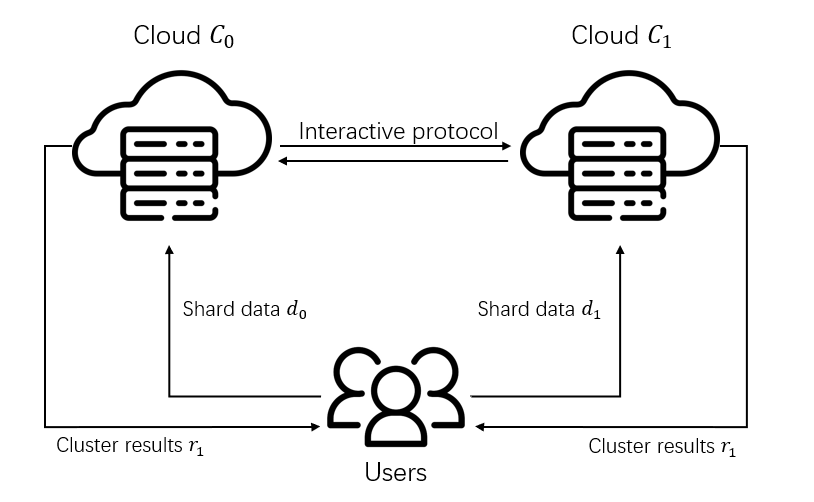
\includegraphics[width=3in]{img/fig5.png}%width=\linewidth
	\caption{System Model}
	\label{sys model}
\end{figure}
如图\ref{sys model}所示,我们的系统由两个部分组成:用户和云服务器。这样的系统模型广泛用于隐私保护研究中\cite{wu2020secure}\cite{bunn2007secure}。这里的客户指的是,持有隐私数据需要聚类来进行数据分析和挖掘的独立用户,他们通常没有足够的计算资源来聚类海量数据,因此需要将计算任务外包以获取结果。常见的实际用户有医疗机构、金融机构等。服务器端通常指的是拥有大量计算资源,提供付费计算服务的云服务器运营厂商例如阿里云、腾讯云等,他们提供机器学习即服务(MLaaS)这一付费模式,用户上传数据后即可离线等待机器学习计算结果。下面我们详细介绍方案中的每一部分:

\begin{itemize}
	\item \textbf{双云服务器}:我们在系统中有两个不共谋的云服务器,标识为$ C_0 $和$ C_1 $,而且均持有用户秘密共享后的数据。他们会在此基础上执行一系列安全协议来实现隐私保护k-means聚类,最后将秘密共享的结果发送给用户。
	\item \textbf{用户}:用户首先在原始数据上构造kd-tree,然后选择随机数来将数据划分为两份秘密共享值,分别发送给双云服务器。在k-means聚类结束后,获取服务器返回的秘密共享结果,运行$ Rec(\cdot,\cdot) $来还原最终结果。
\end{itemize}

\subsection{安全模型}
服务器端与客户端均为半诚实的实体,即二者均会遵循协议内容,不会蓄意停止执行安全协议或是篡改中间计算结果,但会好奇彼此的隐私数据,并尝试从获取的信息中推断其他参与方的信息。虽然云服务器无法还原原始数据,但是可能会企图从计算中间结果中推测数据的分布信息,具体的应对策略为设计安全全面的计算协议,以防止服务器推断原始信息。
\subsection{设计目标}
本节所述隐私保护外包k-means聚类方案设计目标如下:
\begin{itemize}
	\item \textbf{隐私和安全性}:所有外包数据和中间计算结果都不应泄露给双云服务器。同时,服务器无法从秘密共享值推断出原始数据内容以及相关数据特征,例如数据分布。在我们的方案中,上述内容均处于加密状态。
	\item \textbf{高效性}:方案应具备高效性,整个聚类过程主要由双云服务器进行,二者具有丰富的计算和通信资源,能够对海量数据进行处理,极大降低用户计算开销。
	\item \textbf{正确性}:方案应保证计算精度。双云服务器应当能够返回和明文聚类方案一致的计算结果。
\end{itemize}
\section{基于秘密共享的隐私保护计算模块}
\label{s3-mokuai}
为了使用户与云端能够进行安全的交互,我们基于秘密共享技术设计了一系列基本的计算模块。用户通过产生随机值将明文数据拆分为两份密文发送给双云服务器,两方在秘密共享值的基础上进行系列计算和交互,获取最终结果。

\subsection{安全欧式距离计算协议}

计算簇$z$到点$x$之间的欧式距离的计算公式如下:
\begin{equation}
    \label{cal_dist}
    dist=\sqrt{\sum_{j=1}^m\left(z[j]-x[j]\right)^2}
\end{equation}

其中下标$j$标识数据的第$j$个维度,所有数据均为加性秘密共享值。在所有点均被划分到对应簇后,我们通过计算平均值获得簇的中心点。假设簇$z'_i$包含点个数为$|z'_i|$,包含的数据为${x_1,...,x_{|z'_i|}}$,那么簇$z'_i$的中心点计算方式如下:
\begin{equation}
    \label{cal_center}
    z_{i}^{\prime}[j]=\frac{x_{1}[j]+\cdots+x_{\left|z_{i}^{\prime}\right|}[j]}{\left|z_{i}^{\prime}\right|}=\frac{s_{i}^{\prime}[j]}{\left|z_{i}^{\prime}\right|}, 1 \leq j \leq m
\end{equation}

其中$s'_i[j]$表示簇$z'$中所有点第$j$个维度数据之和。在秘密共享值上进行除法比较困难,因此我们采用文献ref-wu中提到的放缩方法来将距离计算中的除法转变为乘法。首先,我们计算全局缩放因子$\alpha$以及簇$z_i$对应的$\alpha_i$,计算方式为:
\begin{equation}
    \label{cal_scale}
    \alpha=\prod_{j=1}^{k}\left|z_{j}\right|, \alpha_{i}=\prod_{j=1 \wedge i \neq j}^{k}\left|z_{j}\right|
\end{equation}

为了方便计算,我们省略公式\ref{cal_dist}中的根号计算,将整个公式改写为:
\begin{equation}
    \label{final_dist_eq}
    dist = \sum_{j=1}^{m}(\alpha x[j] - \alpha_{i}z_i[j])^2
\end{equation}

根据秘密共享方案的性质,我们可以针对公式\ref{final_dist_eq}做出改进,简化计算。在一轮迭代中,无论计算什么距离,缩放因子$\alpha$和$\alpha_i$的值以及相关的计算结果都是不变的,因此我们可以在每轮迭代开始计算这些固定值,减少后续冗余计算。同时,参数不相关的计算可以并行进行,减少云服务器交互的次数。

\subsection{安全比较协议}
安全比较场景如下,参与方$p_i$拥有加性秘密共享值$\langle x_i \rangle$和$\langle y_i \rangle$,其中$i \in \{0, 1\}$,我们希望能够在不泄露$x$和$y$明文值的前提下,获取二者的大小关系$\delta = LT(x, y), \delta = \langle \delta \rangle_0 + \langle \delta \rangle_1$,其中$\delta = LT(x, y)$的具体含义如下:
\begin{equation}
    \operatorname{LT}(x, y)= \begin{cases}1, & \text { if } x<y \\ 0, & \text { if } x \geq y\end{cases}
\end{equation}

在文献ref-crypt中,作者提出了一个高效安全的比较协议来解决百万富翁问题,该方案能够同时比较多对数据,通信开销较小,计算复杂度低。经过多轮不经意传输(oblivious transfer)后,参与方$p_0$和$p_1$分别获得布尔秘密共享结果$\delta = LT(x, y) ,\delta = \langle \delta \rangle^B_0 \bigoplus \langle \delta \rangle^B_1$。

由于本研究中安全比较的输入与输出均为加性秘密共享值,我们在上述百万富翁协议的基础上添加一些改进以构造安全比较协议。具体算法如下:

\begin{algorithm}[htbp]
    \renewcommand{\algorithmicrequire}{\textbf{输入:}}
    \renewcommand{\algorithmicensure}{\textbf{输出:}}
    \caption{SC $\rightarrow (\langle \delta \rangle_0, \langle \delta \rangle_1)$}
    \label{alg_sc}
    \begin{algorithmic}[1]
        \REQUIRE $C_0,C_1$输入$\langle x \rangle_i, \langle y \rangle_i, i\in [0,1]$.
        \ENSURE $C_0,C_1$获得$\langle \delta\rangle_0, \langle \delta\rangle_1$
        \STATE $C_0$ 生成随机数$a, a\in \mathbb{Z}_N$, $\langle r \rangle_0=\langle x \rangle_0-\langle y\rangle_0+a$,将$\langle r \rangle_0$发送给$C_1$
        \STATE $C_1$计算$\langle r \rangle_1 = \langle x \rangle_1-\langle y\rangle_1$,还原$r$值$r=\langle r \rangle_0 + \langle r \rangle_1 = x-y+a$
        \STATE $C_0$和$C_1$使用百万富翁协议来比较$a$和$r$,获得结果$\langle v \rangle_i^B, i\in[0,1]$,$\langle v \rangle_i^B$代表$\langle LT(a,r)\rangle_i^B$
        \STATE $C_i$选择随机数$t_i \in \{0,1\}$,计算$\langle v^{'}\rangle_{1-i}^B=\langle v \rangle_i^B \otimes  t_i$,$C_i$将$\langle v^{'}\rangle_{1-i}^B$发送给$C_{1-i}$,因此$C_0$和$C_1$获取$\langle v \rangle_i^B$的秘密共享值
        \STATE $C_0$和$C_1$计算$\langle\mu \rangle_i^b \leftarrow$ MUL$(\langle v\rangle_1^B,\langle v\rangle_0^B)$
        \STATE 两方计算$ \langle \delta \rangle_i= \langle v \rangle_i^B -  2\langle\mu \rangle_i^B,i\in\{0, 1\}$

    \end{algorithmic}
\end{algorithm}

百万富翁协议无法直接比较秘密共享值,因此我们令云服务器$C_0$产生随机数$a$,将秘密共享值$\langle x \rangle$与$\langle y\rangle$之间的比较转换为明文$a$与$x-y+a$之间的比较。上述转换只需要一轮交互,即可完成。

针对协议的输出,我们需要将布尔秘密共享值($v=\langle v\rangle^B_0 \bigoplus \langle v\rangle^B_1$)转变为加性秘密共享值($v=\langle v\rangle^A_0+\langle v \rangle^A_1$)。根据如下观察,$v^A=\langle v\rangle^B_0+\langle v\rangle^B_1 - 2\langle v\rangle^B_0 \langle v\rangle^B_1$ 即可将布尔共享值转变为加性共享值。为计算$\langle v\rangle^B_0 \langle v\rangle^B_1$,我们令云服务器$C_i$与$C_{1-i}$秘密共享$\langle v \rangle_i^B$,然后进行乘法操作。


\subsection{安全最值计算协议}
安全最值计算协议可以找到一组加性秘密共享值中最值的位置。在$n$个数据中找到最值的传统方式为通过冒泡排序逐个比较大小,从而获得结果。上述方法需要进行$n-1$次比较,并且不能并行计算,效率较低。本文提出的安全比较协议能够并行比较多对数据,基于此,我们针对数据集大小的场景分别设计了两种最值计算协议。

安全最值比较可以分为求解最大值和最小值,方法类似,这里我们以安全求解最小值为例进行阐述,求解最大值只需将协议中求解$LT(x,y)$改为$LT(y,x)$即可。

在处理小数据集时,我们可以通过增加并行比较的数据对,来减少比较的次数。以一个包含三个整数的数据集为例$x_i \in \mathbb{Z}_N, i\in[1,3]$,我们令每个$x_i$与其他两个不同的数据比较。现在我们有6个比较数据对$(x_i, x_{j\neq i}), i,j \in [1,3] $进行一轮数据比较。具体构造流程如下图所示:

\begin{figure}[htbp]
    \centering
    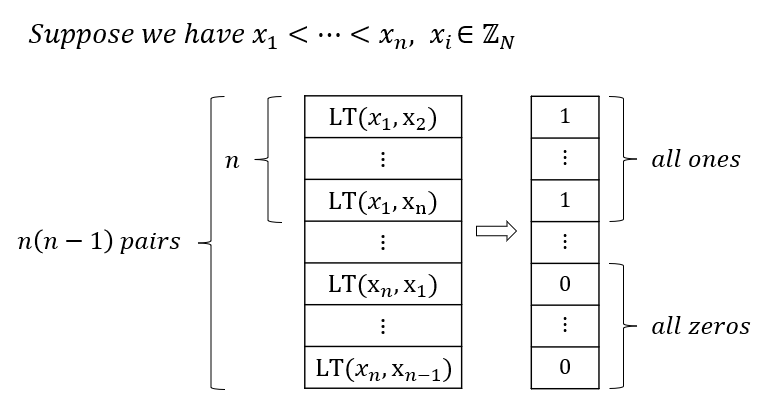
\includegraphics[width=3in]{img/fig4.png}%width=\linewidth
    \caption{Secure minimal on small dataset (SMin(S))}
    \label{smins}
\end{figure}

结果标识为$\{\langle\delta_1\rangle,...,\langle\delta_6\rangle\}$,由云服务器$C_0$和$C_1$秘密共享。然后我们利用MUL来累乘与$x_i$相关的比较结果,获得$\{\langle m_1 \rangle,\langle m_2 \rangle,\langle m_3\rangle\}$。假设$x_1<x_2<x_3$,与$x_1$相关的比较结果全部为$1$,同时与$x_2$,$x_3$相关的比较结果至少包含一个$0$。因此,对应的累乘结果为$m_1=1, m_2=0, m_3=0$。

针对大型数据集,上述方法增加的比较数据对以平方级剧增,带来大量冗余的通信和计算开销。因此,我们放弃增加比较数据对的思路,采取树型结构来减少比较轮次,在冒泡排序需要$n-1$轮比较的基础上,减少为$\log n$轮比较。

假设我们的数据集包含$n$个数据,我们首先比较$n/2$对数据,然后用比较结果与原始数据相乘获取较小值。以$x$,$y$为例,比较结果为$\delta = LT(x,y) $,较小值的计算方式为$r=MUL(\delta, y) + MUL(1-\delta, x)$ 。经过上述操作数据集的大小由$n$变为$n/2$,反复进行上述操作,直到集合仅包含一个数据,即最小值。比较过程如图\ref{sminl}所示。

\begin{figure}[htbp]
    \centering
    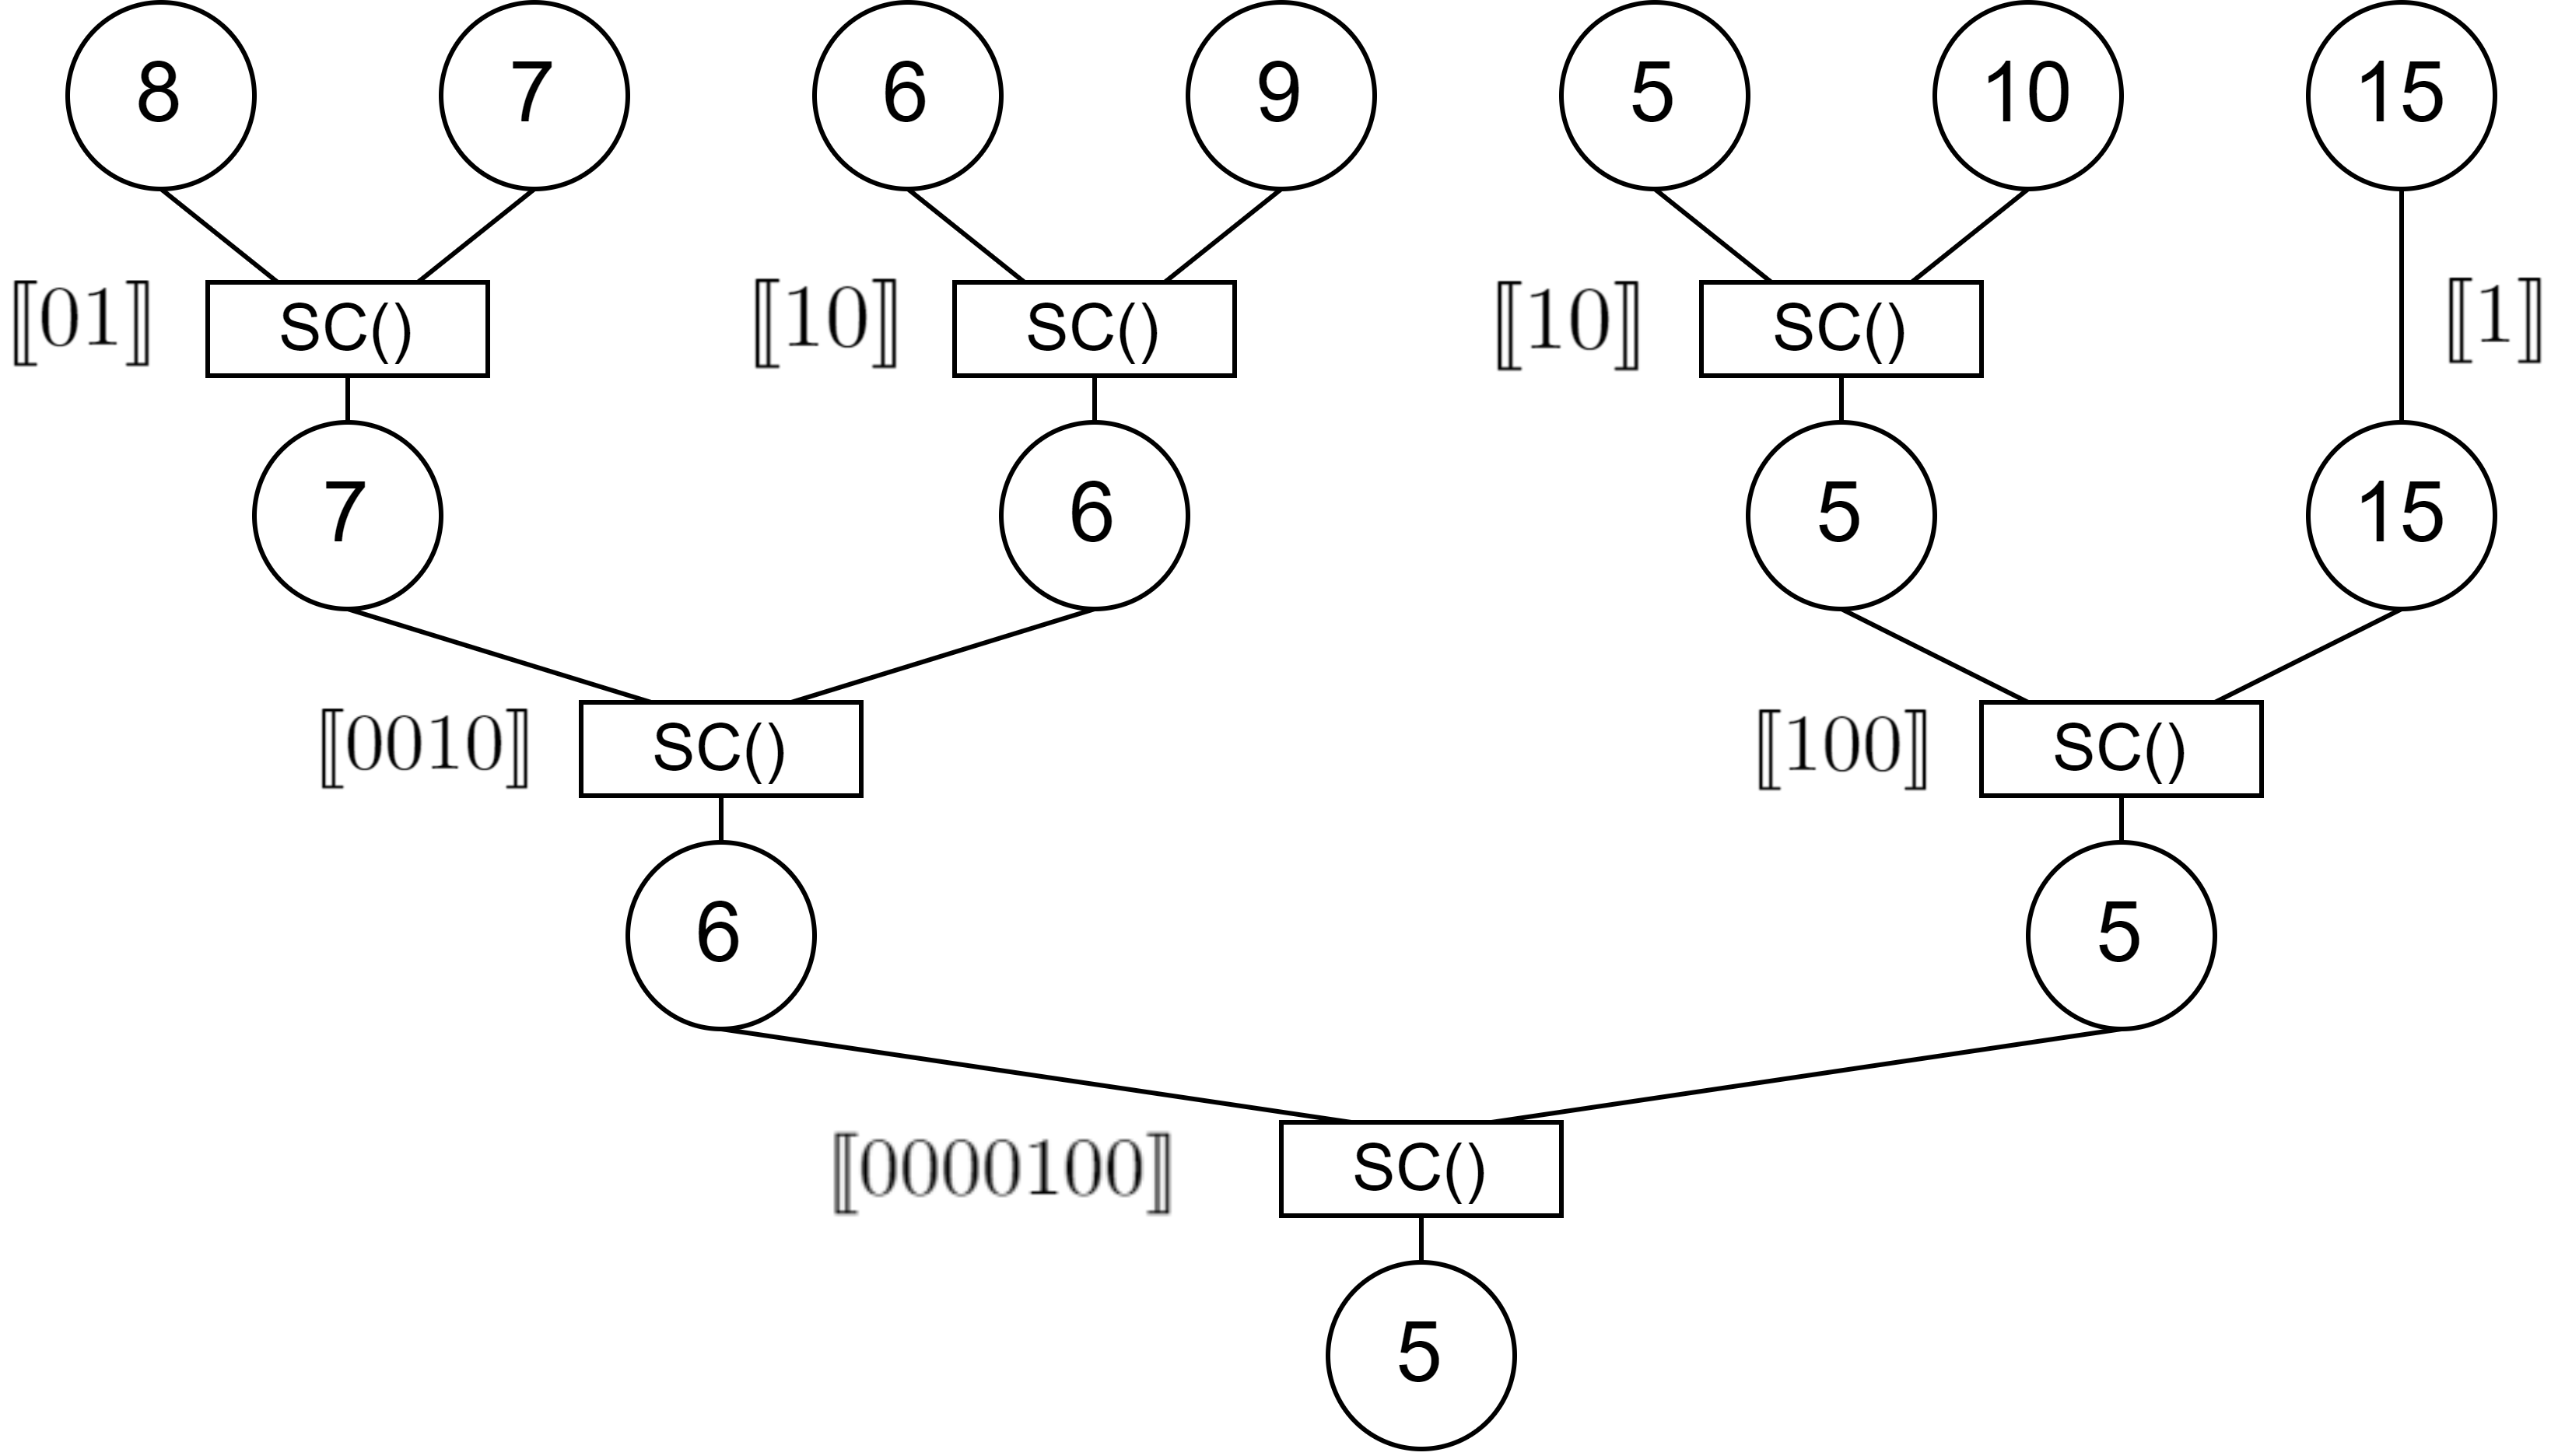
\includegraphics[width=3in]{img/fig1.png}%width=\linewidth
    \caption{Secure minimal on large dataset (SMin(L))}
    \label{sminl}
\end{figure}

\subsection{安全过滤协议}
本节我们将介绍如何在kd-tree数据结构上进行聚类,该方案的正确性验证由ref-kd-tree给出。
自根节点开始,我们依次遍历所有节点来判断当前节点中包含的所有数据点是否可以被划分到某一个簇中。针对每个节点,我们维护一个候选簇集合,该集合中所有簇都可能是节点最终所属簇。在迭代中,我们不断删除不符合条件的候选簇知道仅剩一个候选簇,即节点所属簇。

算法如\ref{alg_sf}所示。2-4行,我们计算kd-tree每个节点到每个候选簇中心的距离,然后借助安全最值协议找到距离最近的候选簇标记为$z^*$。7-12行,我们执行一系列子协议来排除不符合候选条件的簇,即与候选簇$z_j,z_j\neq z^*$相比,节点中包含所有数据点在空间上都离$z^*$更近,则我们认为$z_j$非候选簇。更加详细的规则解释在ref-kd-tree中给出。13-16行,我们执行安全比较协议来判断候选簇集合是否仅剩一个簇。如果是,则将节点中所有数据划分到该候选簇中,并停止向下迭代,否则继续对子节点进行上述操作(17-18行)。若聚类过程即将收敛,那么子节点可以不用进行冗余的距离计算和比较,节省大量计算资源。然而上述方案泄露了一比特数据来判断是否终止子节点迭代,这样少量的数据仅仅轻微泄露了迭代过程的信息,但是带来了效率的巨大提升。ref-p1-35-36中采取了类似的方法作为一个交换来获取性能提升。

\begin{algorithm}[htbp]
    \renewcommand{\algorithmicrequire}{\textbf{输入:}}
    \renewcommand{\algorithmicensure}{\textbf{输出:}}
    \caption{SC $\rightarrow (\langle \delta \rangle_0, \langle \delta \rangle_1)$}
    \label{alg_sf}
    \begin{algorithmic}[1]
        \REQUIRE kd-tree $\langle tr \rangle$以及簇$\langle z \rangle_j, j\in[k]$
        \ENSURE 新的簇中心$\langle z'\rangle_j,j\in[k]$
        \FOR {$i=1$ to $n$}
        \FOR {$j=1$ to $k$}
        \STATE $\langle d \rangle_j \leftarrow$ SED$(\langle z \rangle_j, \langle c \rangle_i)$ %首先计算到每个簇的距离
        \ENDFOR
        \STATE $\{\langle r\rangle_1,...,\langle r\rangle_k\} \leftarrow$ SMin$(\langle d \rangle_1,...,\langle d \rangle_k)$
        \STATE 计算最近候选簇$\langle z^* \rangle \leftarrow \sum_{p=1}^k$MUL$(\langle r \rangle,\langle z\rangle_p)$ %找到最近簇
        \FOR {$j=1$ to $k$} %遍历每个簇
        \STATE $\langle r \rangle \leftarrow$ SC$(\langle u \rangle, 0)$, $\langle \mu \rangle \leftarrow \langle z^{*} \rangle - \langle z\rangle_j$%比较u每个维度和0的大小
        \STATE $\langle v \rangle \leftarrow$ MUL$(\langle r\rangle, \langle c \rangle_{min})+ $MUL$(1-\langle r\rangle,\langle c\rangle_{max})$
        \STATE $\langle d^{*}\rangle \leftarrow$ SED$(\langle z^{*}, \langle v \rangle)$, $\langle d_j \rangle \leftarrow$ SED$(\langle z\rangle_j,\langle v\rangle)$ %如果prune,z_j就是0
        \STATE $\langle r\rangle_j \leftarrow$ SC$(\langle d^{*}\rangle, \langle d\rangle_j)$
        \ENDFOR
        \STATE $\langle f \rangle \leftarrow$ SC$(\sum_{j=1}^{k}\langle r\rangle_j, 1)$
        \IF{$\langle f \rangle_0 + \langle f \rangle_1 == 1$}
        \STATE $\langle \mu \rangle_j \leftarrow \langle \mu \rangle_j +$ MUL$(\langle r\rangle_j, \langle c \rangle),j\in[k]$ %累加
        \ELSE
        \STATE $\langle z \rangle_j \leftarrow$ MUL$(\langle z \rangle_j, \langle r\rangle_j), j\in[k]$
        \STATE pass candidate cluster set $\{\langle z \rangle_1,...,\langle z\rangle_k\}$ to child notes and repeat above process
        \ENDIF
        \ENDFOR

    \end{algorithmic}
\end{algorithm}

\section{基于kd-tree的隐私保护k-means方案}
\label{s3-ppokc}
本节主要介绍基于kd-tree的隐私保护k-means方案(PPOKC)的具体细节。我们假设数据在双云服务器$C_0$和$C_1$上加性秘密共享,并且二者不可以合谋。云服务器在密文基础上进行系列安全协议获取聚类结果,整个过程可以被划分为两个阶段:
\begin{itemize}
    \item \textbf{初始化}:首先,用户基于拥有的明文数据构建kd-tree。然后将数据秘密共享为两份,并分别发送给云服务器$C_0$和$C_1$。此外,原始数据也会在被划分后发送给云服务器以支持其他计算。此后用户不再参与聚类过程。
    \item \textbf{聚类}:对kd-tree中节点执行过滤操作,根节点的候选簇集合包含所有初始簇。针对树中的节点,我们执行过滤操作,直到所有数据都被划分到对应的簇。在每轮迭代结束,我们更新簇中心并且将新簇与旧簇相比较来判断是否满足聚类收敛条件。
\end{itemize}

PPOKC算法的细节在\ref{alg_ppokc}中给出,虽然我们这里提供了一种判断是否停止迭代的方法,在稍后的实验中我们会采取固定迭代次数的方式来测试性能。不同的数据集迭代收敛所需的轮次通常不同,目前大量相关隐私保护聚类研究采取的迭代终止策略通常存在安全问题,即泄露数据集迭代收敛所需轮次。同时,k-means聚类算法在迭代足够多轮次后一定会收敛ref-p1-4。
\begin{algorithm}[htbp]
    \renewcommand{\algorithmicrequire}{\textbf{输入:}}
    \renewcommand{\algorithmicensure}{\textbf{输出:}}
    \caption{SC $\rightarrow (\langle \delta \rangle_0, \langle \delta \rangle_1)$}
    \label{alg_ppokc}
    \begin{algorithmic}[1]
        \REQUIRE 明文数据$x_{ij},i\in[n],j\in[m]$
        \ENSURE 秘密共享的簇中心$\langle z'_j \rangle,j\in[k]$
        \STATE \textbf{初始化(用户)}
        \STATE 在明文基础上构造kd-tree
        \STATE 加性秘密共享数据$x_{ij}$以及kd-tree,随机选择初始簇中心$z_j,j\in[k]$,上述内容分别发送给$C_0$和$C_1$
        \STATE \textbf{聚类($C_0,C_1$)}
        \STATE $\{\langle z^{\prime}_1 \rangle,...,\langle z^{\prime}_k\} \leftarrow$ SF$(\langle z_1\rangle,...,\langle z_k\rangle)$
        \STATE $\langle r \rangle \leftarrow \sum_{i=1}^{n}\sum_{j=1}^{m}$SC$(\langle z_{ij}\rangle-\langle z_{ij}^{\prime}\rangle, 1)$
        \IF{$\langle r \rangle_0 + \langle r\rangle_1 == 1$}
        \STATE 终止迭代,返回结果给用户
        \ELSE
        \STATE $\{\langle z_1 \rangle,...,\langle z_k \rangle \} \leftarrow \{\langle z^{\prime}_1 \rangle,...,\langle z^{\prime}_k\rangle\}$
        \STATE 回到步骤5
        \ENDIF
    \end{algorithmic}
\end{algorithm}

\section{理论分析}
\label{s3-lilun}
\section{实验评估}
\label{s3-shiyan}
\section{本章小结}
\label{s3-xiaojie}